\chapter{Architectural Design}

\section{Overview}
	The application architecture is basically composed by three layers, two of which are provided by Google services as you can see in the following picture:

	\begin{figure}[H]
		\begin{center}
			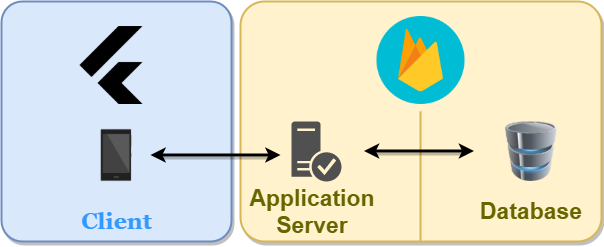
\includegraphics[width=10cm]{img/CookingTime_Architecture.png}
			\caption{Architectural layers}
			\label{Fig:ArchitecturalLayers}
		\end{center}
	\end{figure}

\section{Presentation Layer}
	The presentation layer is figured out by the mobile application which runs on a device and composes the client. 
	It communicates with the Application Server to retrieve and send data according to the user will. 
	The communication is handled by some protected request to the Application Server. 
	The mobile application contains as well most of the logic layer in order to render the data coming from the server and in order to organize the data to be sent.

\section{Application Server}
	This layer is devoted to handle all the information and the request coming from the client side. 
	Moreover it is a sort of bridge between the application and the database. 
	As this layer is hosted by the same provider of the database, the integration is easily implemented and so the communication will be more efficient and safer.

\section{Database Design}
	The database is the one provided by Firebase and it's a NoSQL database, so information are stored in a sort of semi-structured way.
	Using Google solution we can achieve \textbf{Durability and persistence of data} in order to have them always available, 
	\textbf{Consistency} so the database is always in a consistent state, \textbf{Atomicity} in this way all the operation are completely executed and 
	\textbf{Isolation} which means that every operation is executed isolated and independently from the other ones.
	
	\subsection{Database Structure}
	In order to let the reader understand better the structure, here is provided the structure of the NoSQL database used in Firebase, followed by a translated E/R schema of the same database implemented by the application.
	
	\begin{figure}[H]
		\begin{minipage}{0.49\textwidth}
			\dirtree{%
				.1 USER: collection.
				.2 profilePhotoURL: string.
				.2 rating: number.
				.2 recipeNumber: number.
				.2 reviewNumber: number.
				.2 savedRecipes: array<string>.
				.2 userRegisteredWithMail: boolean.
				.2 username: string.				
			}
			\caption{User collection}
		\end{minipage}\hfill
		\begin{minipage}{0.49\textwidth}
			\dirtree{%
				.1 RECIPE: collection.
				.2 author: string.
				.2 category: string.
				.2 description: string.
				.2 difficulty: number.
				.2 imageURL: string.
				.2 INGREDIENT: subcollection.
				.3 name: string.
				.3 quantity: number.
				.3 unit: string.
				.2 isGlutenFree: boolean.
				.2 isLactoseFree: boolean.
				.2 isVegan: boolean.
				.2 isVegetarian: boolean.
				.2 rating: number.
				.2 REVIEW: subcollection.
				.3 author: string.
				.3 comment: string.
				.3 rating: number.
				.3 submissionTime: timestamp.
				.2 reviewNumber: number.
				.2 servings: number.
				.2 STEP: subcollection.
				.3 description: string.
				.3 imageURL: string.
				.3 title: string.
				.2 submissionTime: timestamp.
				.2 subtitle: string.
				.2 time: number.
				.2 title: string.
			}
			\caption{Recipe collection}
		\end{minipage}
	\end{figure}

	\begin{figure}[H]
		\begin{center}
			\centering
			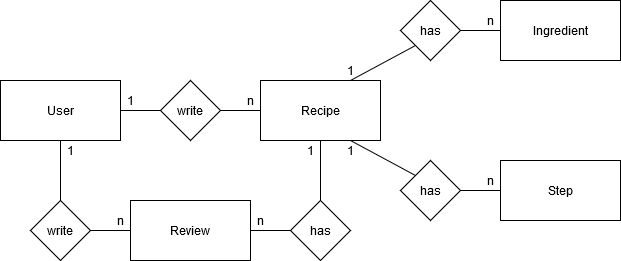
\includegraphics[width=0.8\textwidth]{img/ERDiagram.png}
			\caption{E/R Diagram}
			\label{Fig:ERDiagram}
		\end{center}
	\end{figure}

	\subsection{Database feature}
	The application database allows to:
	
	\begin{itemize}
		\item Login the application.
		\item Read stored data in order to retrieve what was posted by other users.
		\item Data manipulation (CRUD operation) depending on user permissions over data.
	\end{itemize}
	
	
\section{Significative design decision}
\subsection{Login Wrapper}
In order to accomplish the whole implementation of the authentication features we decide to implement a wrapper which is hearing the stream associated to the user object sent by our external services for authetication named Firebase. The component basically provide to the user the signin screen if it is not logged and automatically change the view as soon as the authentication is occured, in this way we don't have to introduce more flags or checks into the code and the application runs more fluently.
\begin{figure}[H]
		\begin{center}
			\centering
			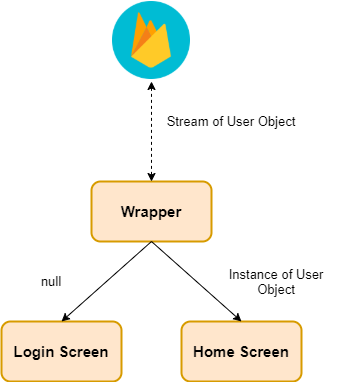
\includegraphics[width=0.8\textwidth]{img/Wrapper.png}
			\caption{Wrapper implementation}
		\end{center}
	\end{figure}
\subsection{Incremental insertion and deletion}
The user is able to modify and insert pictures both for recipe and profile, so in order to prevent having junk data in the databese we decided to implement a routine which is able to detect if a picture is updated with respect to another one, if it occurs then the application delete the picture not in use. That's is very useful as the storing service has limitation over the total amount of free stored data, moreover the performace of the applicatione would be better.